\documentclass[a4paper,10pt,titlepage]{article}

\usepackage{geometry}
\usepackage{amsmath}
\usepackage{amssymb}
\usepackage{txfonts}
\usepackage{microtype}
\usepackage{epsfig}
\usepackage{graphicx}
\usepackage{moreverb}
\usepackage{hyperref}
\usepackage{listings}
\usepackage{xcolor}
\usepackage{textcomp}
\definecolor{listinggray}{gray}{0.98}
\definecolor{lbcolor}{rgb}{0.98,0.98,0.98}
\lstset{
	backgroundcolor=\color{lbcolor},
	tabsize=4,
	rulecolor=,
	language=matlab,
    basicstyle=\scriptsize\ttfamily,
    upquote=true,
    aboveskip={1.5\baselineskip},
    columns=fixed,
    showstringspaces=false,
    extendedchars=true,
    breaklines=true,
    prebreak = \raisebox{0ex}[0ex][0ex]{\ensuremath{\hookleftarrow}},
    frame=single,
    showtabs=false,
    showspaces=false,
    showstringspaces=false,
    identifierstyle=\ttfamily,
    keywordstyle=\color[rgb]{0,0,1},
    commentstyle=\color[rgb]{0.133,0.545,0.133},
    stringstyle=\color[rgb]{0.627,0.126,0.941},
}
\usepackage{eso-pic}
\usepackage{ifthen}

\AddToShipoutPictureBG{\ifthenelse{\equal{\value{page}}{0}}{}{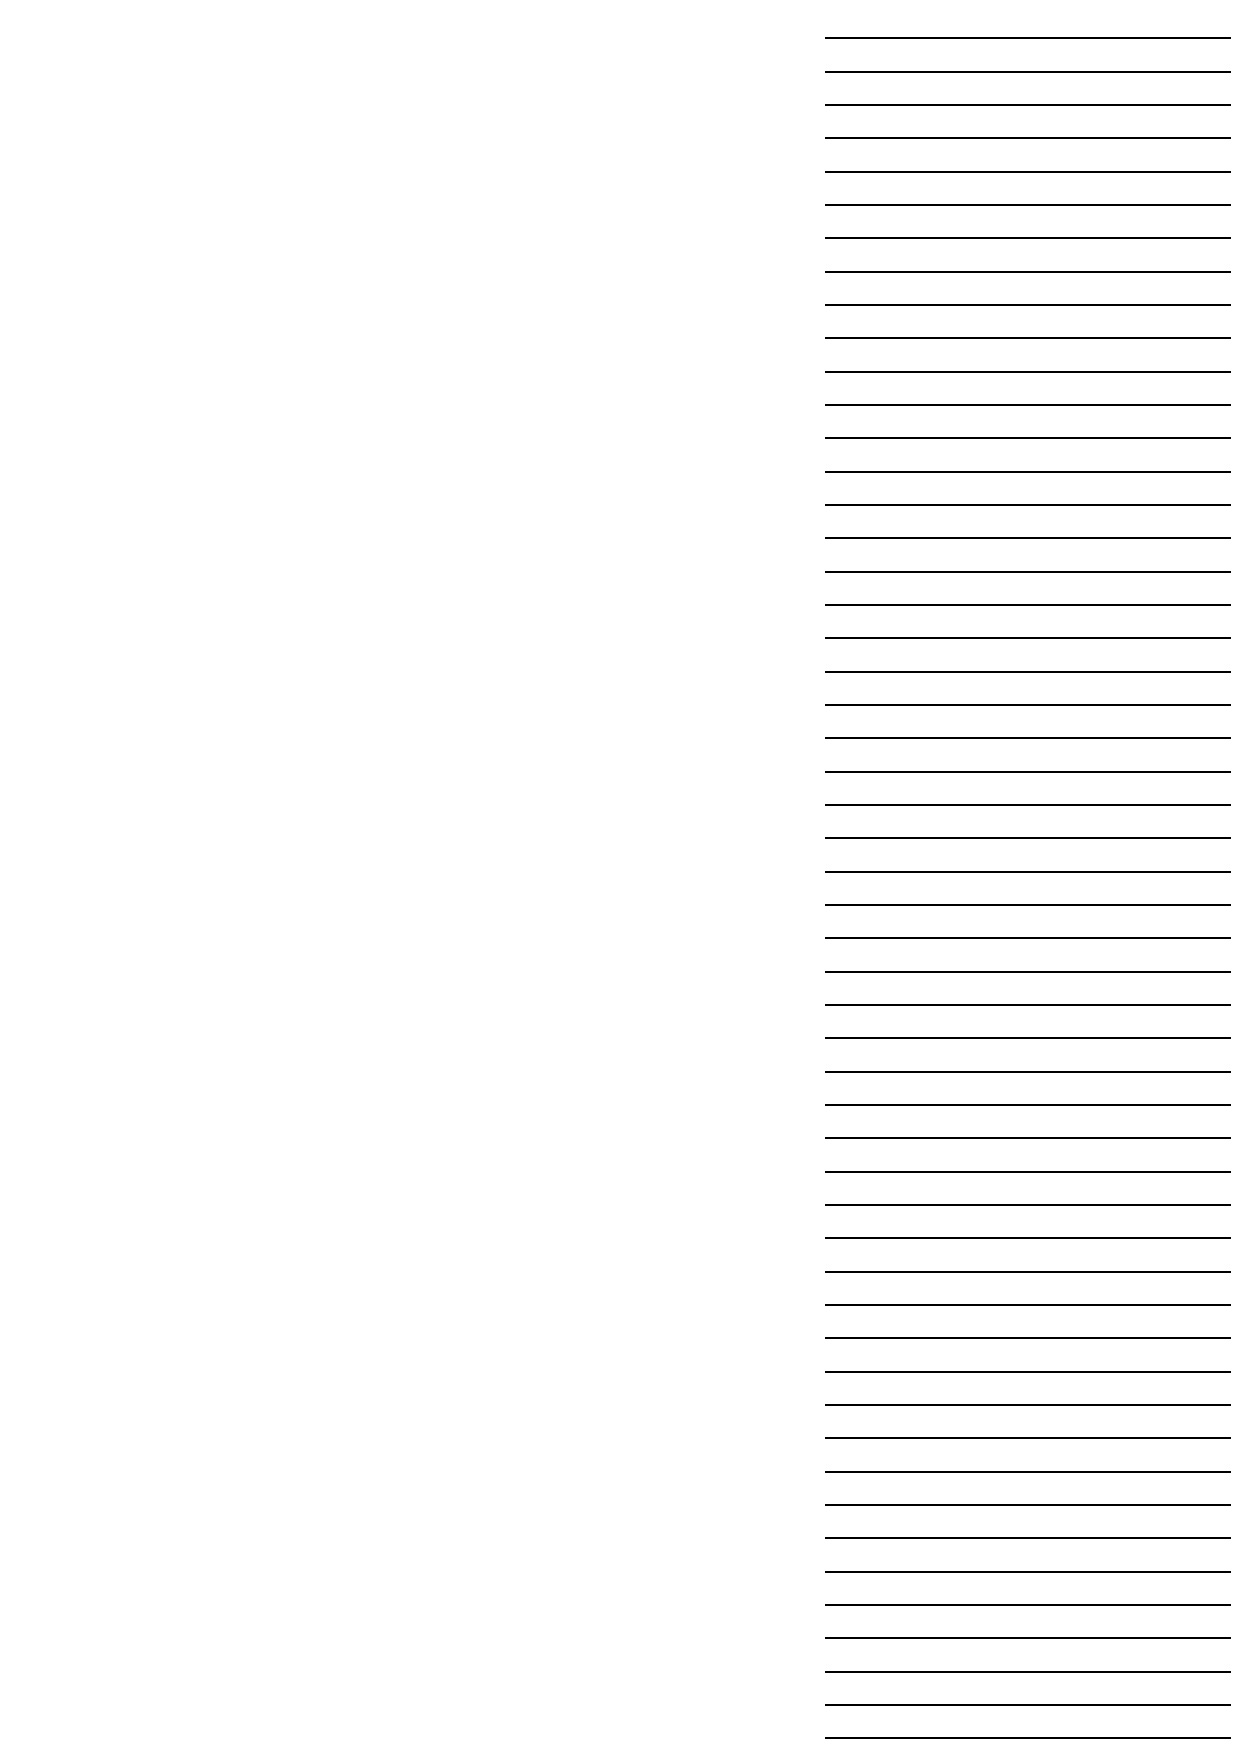
\includegraphics{template_files/backgroundlines}}}


\usepackage{tikz}
\usepackage{pgfplots}
\usepackage{tikzscale}
\usepackage{graphicx}
\usepackage{float}
\usepackage{subcaption}
\usepackage{comment}
\usepackage{units}
\usetikzlibrary{external}\tikzexternalize


\title{H2b: Variational Monte Carlo}
\author{Victor Nilsson and Simon Nilsson (930128-1854)}
\date{\today}

\begin{document}

\newgeometry{top=2cm,bottom=2cm,left=2cm,right=2cm}

\begin{titlepage}

\setcounter{page}{0}

\begin{center}
{\huge \bf \color{red} NB: The graded, first version of the report must be
                           returned if you hand in a second time! } \\
\vspace{3cm}
\makeatletter
{ \huge \@title } \\
\vspace{1cm}
{ \Large \@author }\\
\vspace{1cm}
{ \Large \@date }\\
\makeatother
\end{center}

\vfill

\begin{flushright}
{\Large
\begin{tabular}{|c|c|c|}
\hline
Task N\textsuperscript{\underline{o}} & Points & Avail.\ points \\ \hline
\hspace{3cm} & \hspace{3cm} & \hspace{3cm} \\ \hline
~ & ~ & ~ \\ \hline
~ & ~ & ~ \\ \hline
~ & ~ & ~ \\ \hline
~ & ~ & ~ \\ \hline
~ & ~ & ~ \\ \hline
~ & ~ & ~ \\ \hline
~ & ~ & ~ \\ \hline
$\sum$ & ~ & ~ \\
\hline
\end{tabular}}
\end{flushright}

\end{titlepage}

\newgeometry{top=2cm,bottom=2cm,left=1.5cm,right=7.4cm}


\section*{Introduction}

In quantum mechanics we often have a Hamiltonian operator $\mathbf{H}$ that describes the energy of the studied system. Given a wave function $\psi$, the corresponding energy for that state is given by,

\begin{equation}
E=\frac{\left<\psi|\mathbf{H}|\psi\right>}{\left<\psi|\psi\right>}.
\end{equation}

For the Hamiltonian we have a corresponding ground state energy $E_0$ which is the lowest energy possible. The wave function $\psi_0$ that represents this lowest energy is often not known and a trial wave function $\phi$ is guessed. For any such $\phi \neq \psi_0$, the energy given by the Hamiltonian will always be larger than the ground state energy, $E \geq E_0$. For the next few problems we want to study the Hamiltonian describing the energy of a helium atom with two electrons. This Hamiltonian, neglecting fine structure, have the following form,
\begin{equation}
\mathbf{H}=-\frac{\hbar}{2m_e}\left(\nabla_1^2+\nabla_2^2\right)-\frac{e^2}{4\pi \epsilon_0}\left(\frac{2}{r_1}+\frac{2}{r_2}-\frac{1}{|r_1-r_2|}\right),
\end{equation} 
where $m_e$ is the mass of a electron, $e$ is the elementary charge, $\hbar$ is the reduced Planck constant, $\epsilon_0$ is the vacuum permittibility, $r_1$ and $r_2$ are the distances of the two electrons from the nucleus and the distance between these is $|\mathbf{r}_1-\mathbf{r}_2|$. For simplicity we use atomic units, i.e. $\hbar=e=m=4\pi\epsilon=1$. We want to see how well the trial wave,
\begin{equation}
\psi_T(\mathbf{r_1},\mathbf{r_2})=e^{-2r_1}e^{-2r_2}e^{r_{12}/2(1+\alpha r_{12})},
\end{equation}

is compared to the unknown ground state wave function $\psi_0$, where $\alpha$ is a parameter to be optimized. To calculate the energy for this trial wave we need to integrate over the whole physical line in 6 dimensions. This cannot be done analytically and we need to use numerical approximation methods to evaluate the integral. We will use the variational Monte Carlo method using the Metropolis algorithm. For each state $(\mathbf{r_1},\mathbf{r_2})$ we thus have the \textit{local energy},
\begin{equation}
E_{L}(\mathbf{r}_1,\mathbf{r}_2)= \frac{\mathbf{H}\psi_L(\mathbf{r}_1,\mathbf{r}_2)}{\psi_L(\mathbf{r}_1,\mathbf{r}_2)}
\end{equation}
and the normalised probability to be in this state is,
\begin{equation}
\rho(\mathbf{r}_1,\mathbf{r}_2)=\frac{|\psi_L(\mathbf{r}_1,\mathbf{r}_2)|^2}{\int dr_1dr_2|\psi_L(\mathbf{r}_1,\mathbf{r}_2)|^2}.
\end{equation}

This probability will never be calculated directly as we only need the relative probabilities from the current state to a new state,
\begin{equation}
\rho_{rel}(\mathbf{r'}_1,\mathbf{r'}_2,\mathbf{r}_1,\mathbf{r}_2)=\frac{|\psi_L(\mathbf{r'}_1,\mathbf{r}_2')|^2}{|\psi_L(\mathbf{r}_1,\mathbf{r}_2)|^2}.
\end{equation}


\section*{Problem 1}

\begin{figure}[H]
    \centering
    \captionsetup[subfigure]{justification=centering}
    \begin{subfigure}[b]{0.48\textwidth}
        \centering
        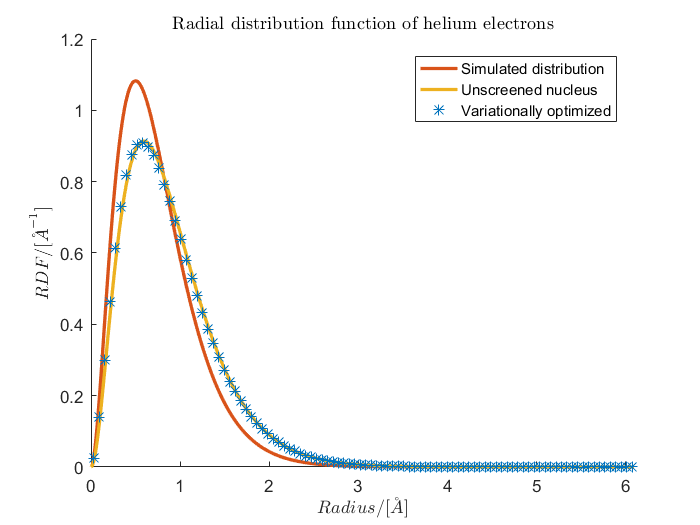
\includegraphics[width=\textwidth]{graphics/task1/radius.png}
    \end{subfigure}
    \begin{subfigure}[b]{0.48\textwidth}
        \centering
        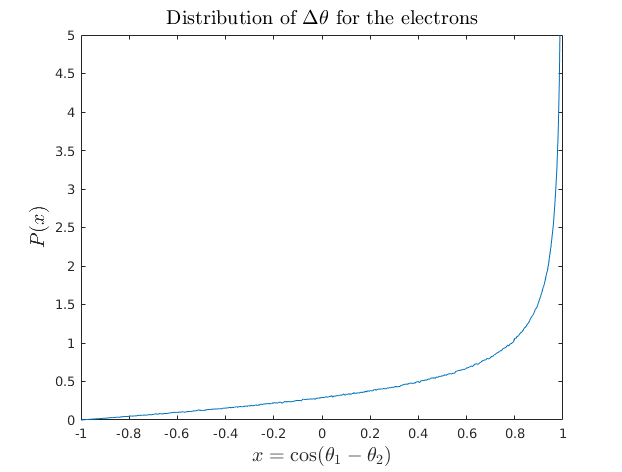
\includegraphics[width=\textwidth]{graphics/task1/angle_diff_dist.png}
    \end{subfigure}
    \caption{\textit{Left:} Simulated and calculated radial distribution function for the two electrons in the helium atom. \textit{Right:} The distribution of cosine of the angle $\theta$ between the two electrons.}
    \label{fig:RDF}
\end{figure}

In this problem we studied a He atom using the variational Monte Carlo method with the Metropolis algorithm. In the Metropolis algorithm a new trial state is obtained by randomly displacing both electrons in all three dimensions simultaneously. The displacement is bounded by a cube with side $d$, where $d$ is a simulation parameter which was chosen as $\unit[1]{\AA}$. Other equations used can be found in \cite{probdesc}.

From the obtained sample points, a radial probability distribution function could be approxiated, which can be seen in Fig.~\ref{fig:RDF} (left). Comparing the result to the variationally optimized distribution and the central field approximation result we conclude that that the results are the same as the variationally optimized distribution and that the method is working properly. This effect is due to screening, causing the effective nucleus charge to be lower than the actual charge.

From these sample points we can also study the correlation of the angle between the two electrons, $\theta$. We obtain $\theta$ by using the relation
\begin{equation}
\theta = \arccos \left( \frac{\mathbf{r}_1 \cdot \mathbf{r}_2}{|\mathbf{r}_1| |\mathbf{r}_2|} \right).
\end{equation}
As stated in \cite{probdesc}, if they are uncorrelated, i.e. equally distributed over the unit sphere, then the probability distribution would be $P(\theta) = \sin \theta / 2$ for $0 < \theta < \pi$, or
\begin{equation}
	x = \cos \theta \Rightarrow P(x) = \frac{1}{2},\quad -1 < x < 1.
\end{equation}

The variational Monte Carlo yields the results in Fig.~\ref{fig:RDF} (right). This indicates a clear correlation where the electrons tend to be approximately on the opposite side of the nucleus. At least a slight correlation is expected, however whether it should be this strongly correlated or not, we do not know.

The mean energy obtained with variational Monte Carlo was -2.877 in Hartree atomic units. The results from mean-field approximation, for unscreened and screened nucleus respectively, are -2.75 and -2.85 atomic units. We see that the results are similar and that the one obtained with variational MC is even lower than the others and is therefore probably closer to the ground-state energy for Helium.


\section*{Problem 2}

\begin{figure}[H]
	\centering
	\captionsetup[subfigure]{justification=centering}
	\begin{subfigure}[b]{0.48\textwidth}
		\centering
		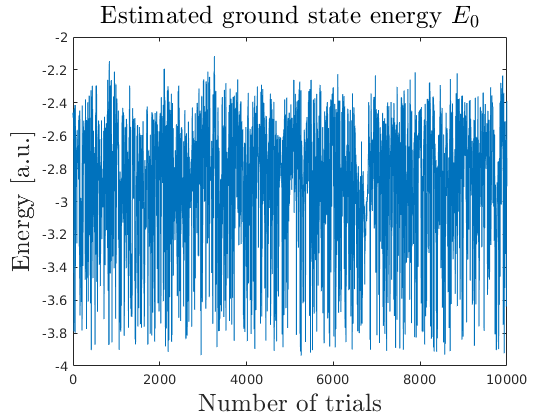
\includegraphics[width=\textwidth]{graphics/task2/local_energy.png}
	\end{subfigure}
	\begin{subfigure}[b]{0.48\textwidth}
		\centering
		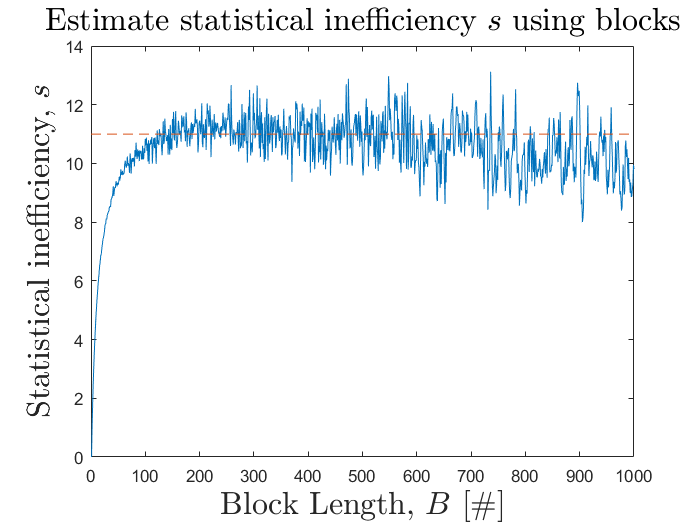
\includegraphics[width=\textwidth]{graphics/task2/block_error.png}
	\end{subfigure}
	\caption{\textit{Left:} The estimation of the ground state energy $E_0$ for different number of trials without equilibration, there is not much deviation in the energy for $\approx10^4$ trials. \textit{Right:} Estimation of the statistical inefficiency based on different block lengths. After the length of about 200 we can see that the statistical inefficiency $s$ deviates around 11 and starts to go slightly down for higher lengths.}
	\label{fig:block_error}
\end{figure}

In order for the Metropolis algorithm to yield good and accurate results we need the system to run for a time in order to reach statistically likely configurations as the initial condition might be very unlikely. We can see in Fig. \ref{fig:block_error}(left) that we need discard $\approx10^4$ trials. For the remainder of the tasks we go well beyond this number, we take one tenth of the total trials as equilibration, to really make sure we reach a good statistically likely Markov chain.

When we know where to start our simulation we need to know how correlated the trial data is in order to receive accurate statistics. If we take the energy in each time-step we would like to know it's statistical inefficiency. This calculation is done in two ways to show our results are rigorous, first by considering blocks of different lengths and calculate the correlation of the data in these blocks, and secondly by calculating the auto-correlation function.

The results for using the block length can be seen in Fig.\ref{fig:block_error}(right) and we see that it stagnates around 11 for about 200 in block length. The statistical inefficiency using the auto-correlation was also 11.




\section*{Problem 3}


\begin{figure}[H]
	\centering
	\captionsetup[subfigure]{justification=centering}
	\begin{subfigure}[b]{0.48\textwidth}
		\centering
		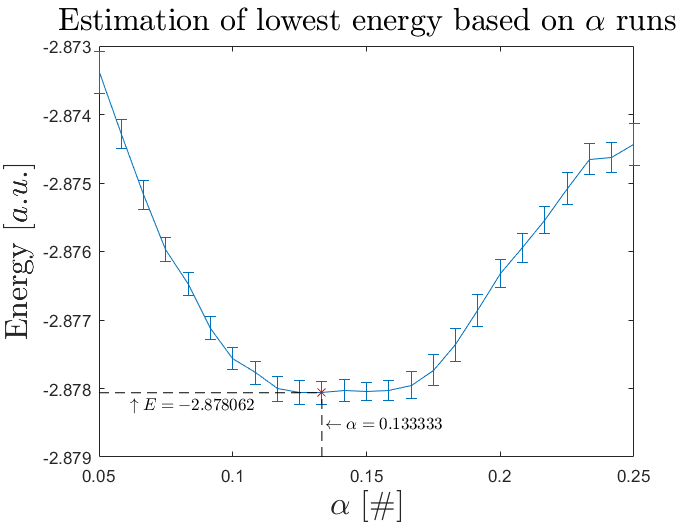
\includegraphics[width=\textwidth]{graphics/task3/lowest_energy_indep_alpha.png}
	\end{subfigure}
	\begin{subfigure}[b]{0.48\textwidth}
		\centering
		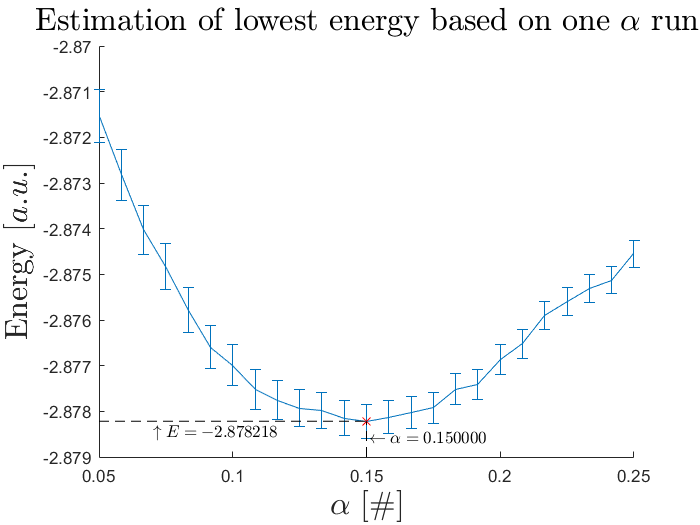
\includegraphics[width=\textwidth]{graphics/task3/lowest_energy_one_alpha_run.png}
	\end{subfigure}
	\caption{Estimation of the optimal variation parameter $\alpha$ for calculating the lowest energy in the Metropolis algorithm. This estimation is done by running several independent runs for each $\alpha$ (\textit{left}) and also using a long simulation with only one run per $\alpha$ (\textit{right}).}
	\label{fig:optimize_alpha}
\end{figure}

In order to determine the best value of the variational parameter $\alpha$, we run the Metropolis using several different $\alpha$ values in the interval $0.05 \leq \alpha \leq 0.25$. We estimate the $\alpha$ dependence in two ways, first by doing short independent runs for the same $\alpha$ and estimating the mean and standard deviation from the average energies of the individual runs, see Fig.~\ref{fig:optimize_alpha} (\textit{left}). The second way we do by taking a long run, about $100$ times longer than the short ones, and estimating the mean and standard deviation of the energy on the single run over time, see Fig.~\ref{fig:optimize_alpha} (\textit{right}). 

\section*{Problem 4}

Instead of guessing the optimal $\alpha$ we can instead use a damped steepest decent to reach a local minimum for the $\alpha$. Here we use the update rule in the method,
\begin{equation}
\alpha_{p+1} = \alpha_p-\gamma_p \nabla_\alpha E(\alpha_p)
\end{equation} 
where the damping coefficient,
\begin{equation}
\gamma_p=Ap^{-\beta},
\end{equation}
with $A=1$ and $0.5\leq\beta < 1$. The gradient $\nabla_\alpha E(\alpha)$ is calculated to,
\begin{equation}
\nabla_\alpha E(\alpha) = 2\left[\left<E_L(\mathcal{R})\nabla_\alpha \ln{\psi_T(\mathcal{R})}\right>-\left<E_L(\mathcal{R})\right>\left<\nabla_\alpha\ln{\psi_T(\mathcal{R})}\right>\right]
\end{equation}
where $\mathcal{R}$ is the electron state configurations and the averages are calculated in the ordinary Metropolis algorithm. The gradient on the $wave function $ is,
\begin{equation}
\nabla_\alpha \ln{\psi_T(\mathcal{R})} = -\frac{r_{12}^2}{2(1+\alpha r_{12})^2}.
\end{equation}

Using this method, and with $\beta = 0.75$ we find that the minimum energy to be $E_{min}=-2.891$ with the corresponding $\alpha$ as $\alpha_{min}=0.1426$. This found $\alpha$ lies between the two results gained in Problem 3.

\begin{table}[H]
	\centering
	\caption{Put some capton here.}
	\begin{tabular}{|l|cc|}
		\hline $\beta$ & $\alpha$ & $Energy_{min}$ \\ \hline
		 0.5 & 0.1434688 & -2.893317 \\ \hline
		 0.625 & 0.1434688 & -2.893317 \\ \hline
		 0.75 & 0.1431064 & -2.892874 \\ \hline
		 0.875 & 0.1427814 & -2.893997 \\ \hline
	\end{tabular}
	\label{tab:prob5}
\end{table}


\section*{Problem 5}

Using the $\alpha$ found in Problem 4, we do a long simulation in order to see what value we receive. We find our energy to be, $E_{min}=-2.878223$ which lies between the Hartree value $\unit[-2.862]{a.u.}$ and the experimental number $\unit[-2.9033]{a.u.}$

$Mean = -2.878153, var = 1.275041E-7$


\bibliography{references}
\bibliographystyle{plain}


\appendix
\section{Source code}
\subsection{\texttt{helper.c}}
\lstinputlisting[language=c, numbers=left]{../code/helper.c}

\subsection{\texttt{rng\_gen.c}}
\lstinputlisting[language=c, numbers=left]{../code/rng_gen.c}

\subsection{\texttt{Task1/main.c}}
\lstinputlisting[language=c, numbers=left]{../code/Task1/main.c}

\subsection{\texttt{Task2/main.c}}
\lstinputlisting[language=c, numbers=left]{../code/Task2/main.c}

\subsection{\texttt{Task3/main.c}}
\lstinputlisting[language=c, numbers=left]{../code/Task3/main.c}

\subsection{\texttt{Task4/main.c}}
\lstinputlisting[language=c, numbers=left]{../code/Task4/main.c}

\subsection{\texttt{Task5/main.c}}
\lstinputlisting[language=c, numbers=left]{../code/Task5/main.c}


\end{document}
